
% This LaTeX was auto-generated from MATLAB code.
% To make changes, update the MATLAB code and republish this document.

\documentclass{article}
\usepackage{graphicx}
\usepackage{color}

\sloppy
\definecolor{lightgray}{gray}{0.5}
\setlength{\parindent}{0pt}

\begin{document}

    
    \begin{verbatim}
function secondTask
A = [0, 1; 0, -3];%матрица от коефициенти
B = [0;1];
y0 = [0;0]; % начални условия
h = 0.1; % стъпка
n = 200; % итерации
x1 = 0; x(1)=0; y1(1)=0; y2(1)=0;
A2=expm(A*h);
for i=2:n
     y=A2*y0+(h/2)*(A2*B*myFunction(x1))+(B*myFunction(x1+h));
     y1(i)=y(1); y2(i)=y(2);
     y0=y;
     x1 = x1+h; x(i)=x1;
end
figure(3), plot(x,y1,x,y2);
xlabel('x');
ylabel('y');
legend('y_1', 'y_2', 'Location', 'best', 'Orientation', 'vertical');
title('Решение по метода на матрична експонента');
end

function f = myFunction(x)
f = x*exp(-2*x);
end
\end{verbatim}

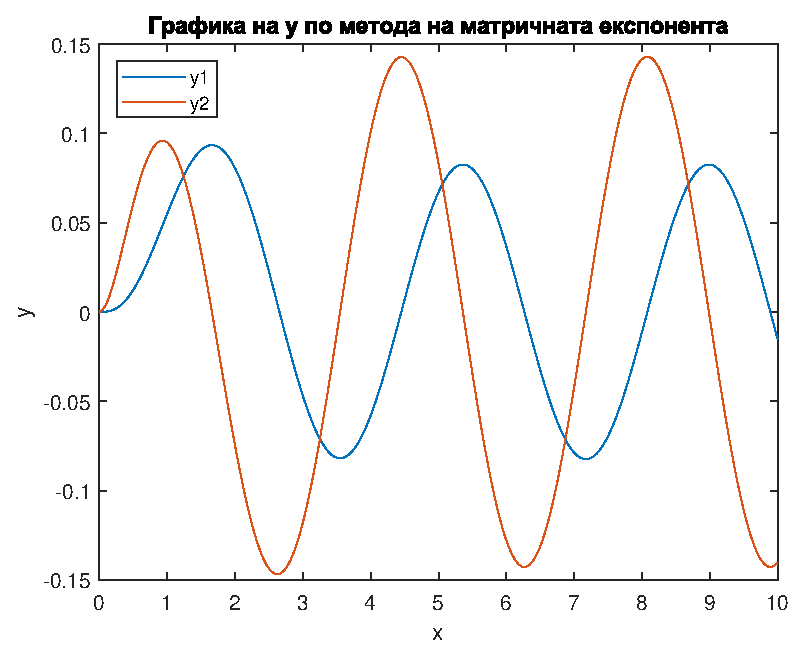
\includegraphics [width=4in]{secondTask_01.eps}



\end{document}

